\documentclass[12pt, a4paper, simple]{eskdtext}

\usepackage{hyperref}
\usepackage{env}
\usepackage{_sty/gpi_lst}
\usepackage{_sty/gpi_toc}
\usepackage{_sty/gpi_t}
\usepackage{_sty/gpi_p}
\usepackage{_sty/gpi_u}

% Код
% \ESKDletter{О}{Л}{Р}
% \def \gpiDocTypeNum {81}
% \def \gpiDocVer {00}
% \def \gpiCode {\ESKDtheLetterI\ESKDtheLetterII\ESKDtheLetterIII.\gpiStudentGroupName\gpiStudentGroupNum.\gpiStudentCard-0\gpiDocNum~\gpiDocTypeNum~\gpiDocVer}

\def \gpiDocTopic {Отчёт лабораторной работы №\gpiDocNum}


% колонтитулы
\usepackage{fancybox, fancyhdr}
\fancypagestyle{plain}
{
    \renewcommand{\footrulewidth}{0pt}          % Толщина отделяющей полоски снизу
    \renewcommand{\headrulewidth}{0pt}          % Толщина отделяющей полоски сверху
    % \fancyhead[C]{\hfill\gpiCode\hfill}         % Коллонтитул сверху
    \fancyfoot[C]{\hfillстр.~\thepage}          % Коллонтитул снизу
}

% Графа 1 (наименование изделия/документа)
% \ESKDcolumnI {\ESKDfontII \gpiTopic \\ \gpiDocTopic}

% Графа 2 (обозначение документа)
% \ESKDsignature {\gpiCode}

% Графа 9 (наименование или различительный индекс предприятия) задает команда
% \ESKDcolumnIX {\gpiDepartment}

% Графа 11 (фамилии лиц, подписывающих документ) задают команды
% \ESKDcolumnXIfI {\gpiStudentSurname}
% \ESKDcolumnXIfII {\gpiTeacherSurname}
% \ESKDcolumnXIfV {\gpiTeacherSurname}

\begin{document}
    \begin{ESKDtitlePage}
    \ESKDstyle{empty}
    \begin{center}
        \gpiMinEdu \\
        \gpiEdu \\
        \gpiKaf \\
    \end{center}

    \vfill

    \begin{center}
        \gpiTopic
    \end{center}

    \vfill

    \begin{center}
        \textbf{\gpiDocTopic} \\
        ПО ДИСЦИПЛИНЕ \gpiDiscipline \\
    \end{center}

    \vfill

    \begin{flushright}
        \begin{minipage}[t]{7cm}
            Выполнил:\\
            \PageTitleStudentInfo
            \PageTitleDateField
            \hspace{0pt}

            Проверил:\\
            \PageTitleTeacherInfo
            \PageTitleDateField
        \end{minipage}
    \end{flushright}

    \vfill

    \begin{center}
        \PageTitleCity~\ESKDtheYear
    \end{center}
\end{ESKDtitlePage}

    \ESKDstyle{empty}
    \thispagestyle{plain}
    \pagestyle{plain}

    % \paragraph{}
    \begin{center}
        \textbf{\gpiDocTopic}
    \end{center}

    % = = = = = = = =
    \paragraph{} \textbf{Тема}: <<\gpiTopicRep>>

    \paragraph{} \textbf{Цель}: Разработка приложения, демонстрирующего геолокационные возможности.

    \paragraph{} \textbf{Что нужно сделать}:
    Создать Android приложение, которое отображает сообщение, что GPS включён или выключен.
    При включённом GPS показывать ширину, долготу и время определения.

    \paragraph{} \textbf{Разработка дизайна}:

    \begin{figure}[!h]
        \centering
        \begin{minipage}{0.19\textwidth}
            \centering
            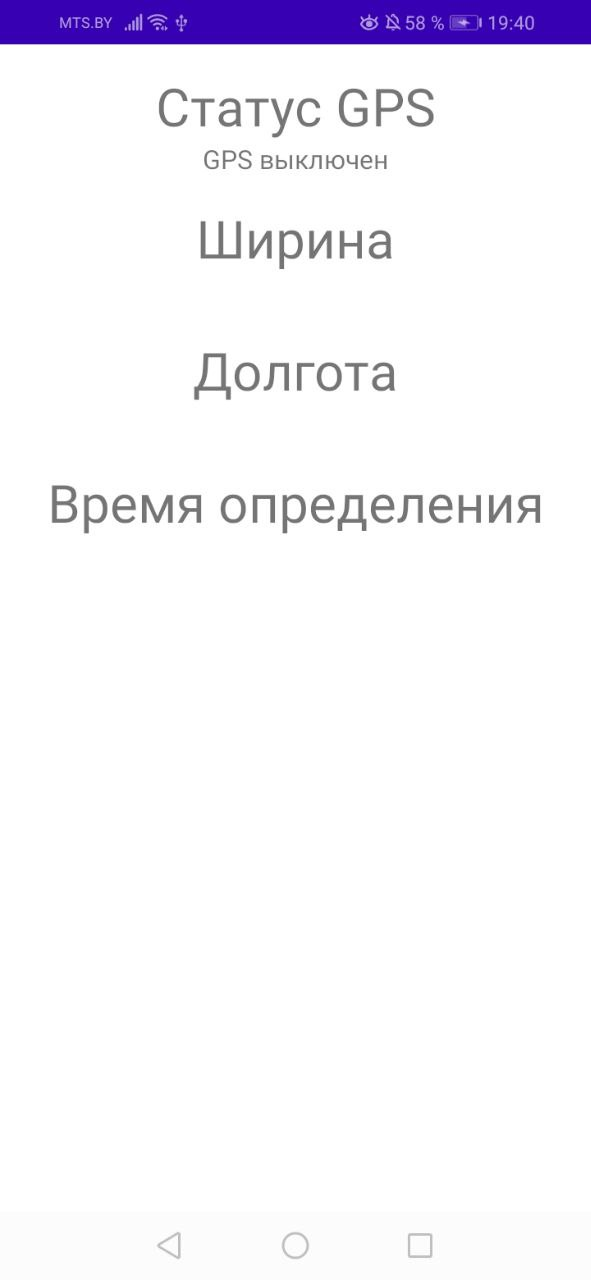
\includegraphics[width=\linewidth]
                {_assets/gps_off.jpg}
            \caption{GPS выключен}
            \label{fig:i_draw_1}
        \end{minipage}
        \begin{minipage}{0.19\textwidth}
            \centering
            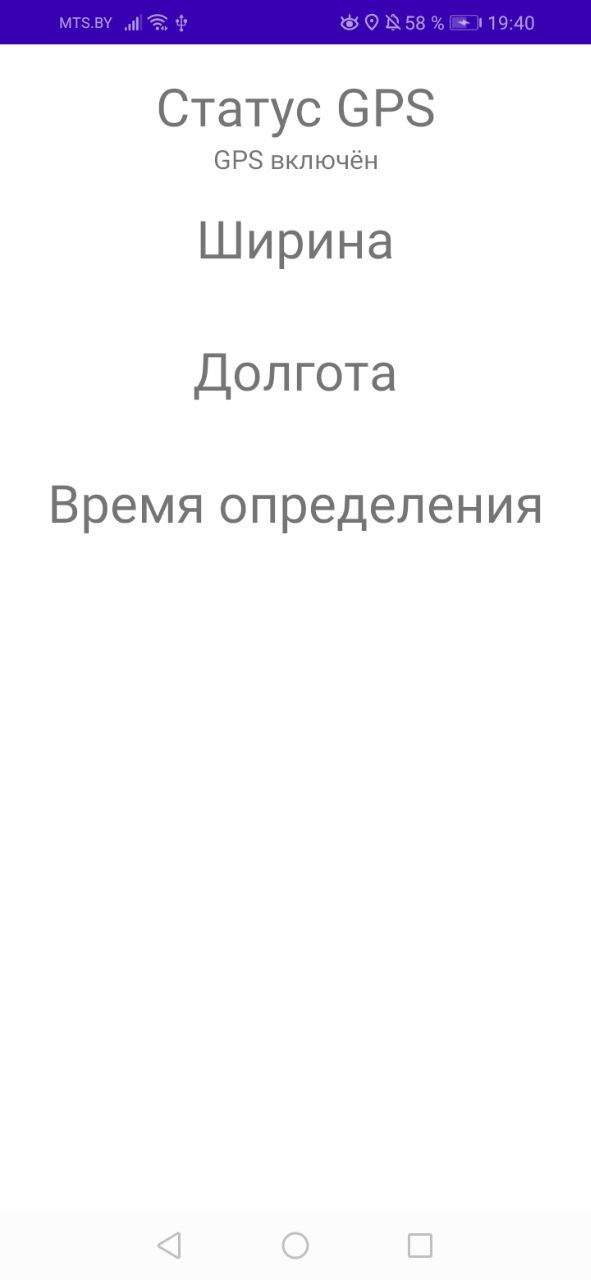
\includegraphics[width=\linewidth]
                {_assets/gps_on.jpg}
            \caption{GPS включён}
            \label{fig:i_draw_2}
        \end{minipage}
        \begin{minipage}{0.19\textwidth}
            \centering
            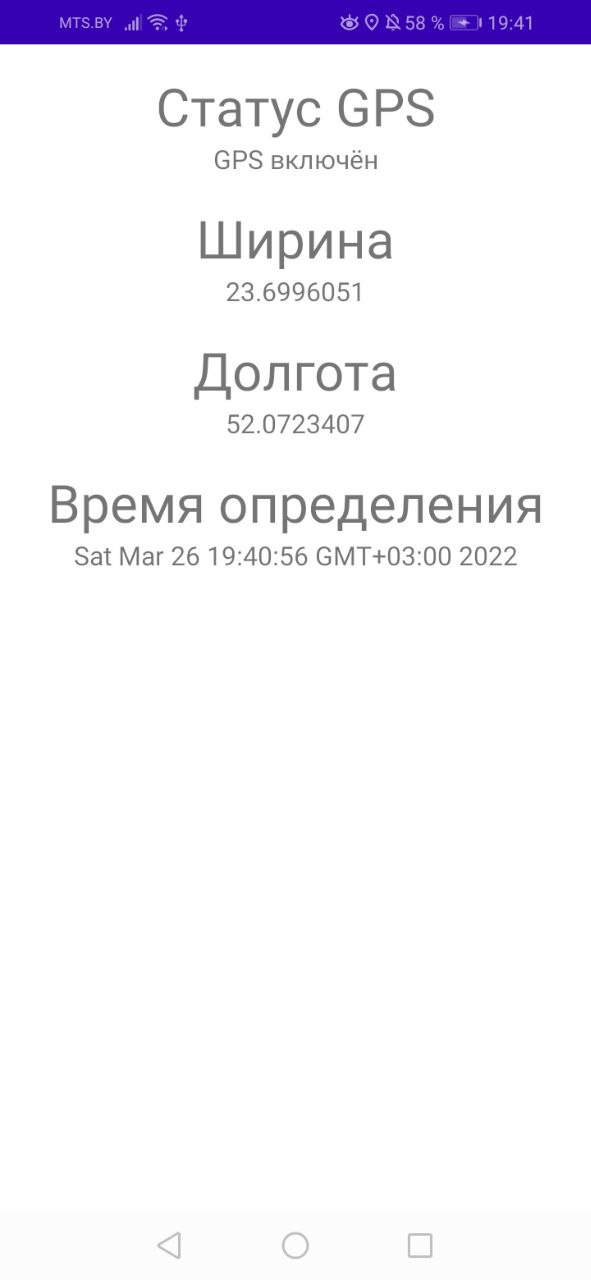
\includegraphics[width=\linewidth]
                {_assets/gps_1.jpg}
            \caption{GPS спустя 40 секунд}
            \label{fig:i_draw_3}
        \end{minipage}
        \begin{minipage}{0.19\textwidth}
            \centering
            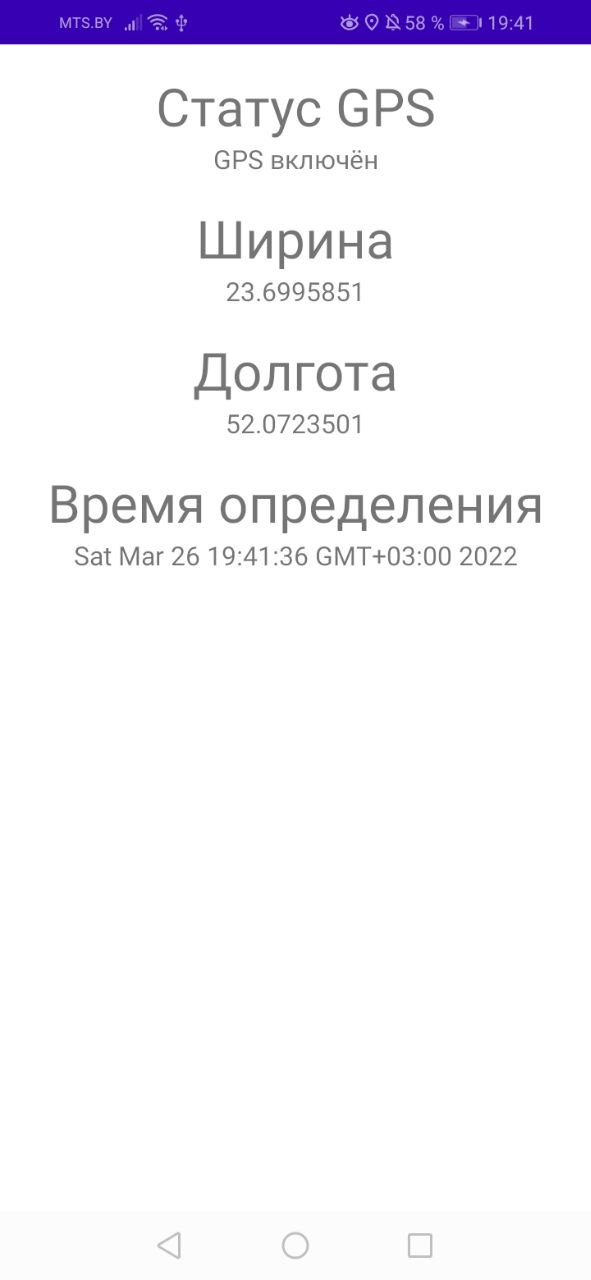
\includegraphics[width=\linewidth]
                {_assets/gps_2.jpg}
            \caption{GPS спустя 40 секунд}
            \label{fig:i_draw_S}
        \end{minipage}
        \begin{minipage}{0.19\textwidth}
            \centering
            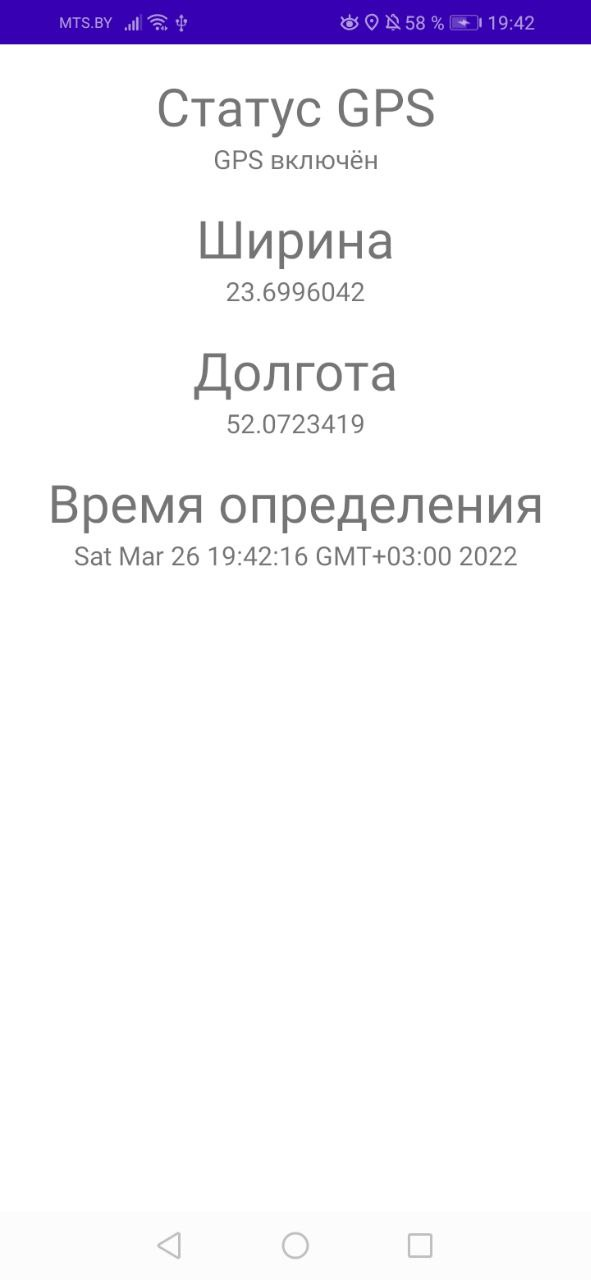
\includegraphics[width=\linewidth]
                {_assets/gps_3.jpg}
            \caption{GPS спустя 40 секунд}
            \label{fig:i_draw_S}
        \end{minipage}
    \end{figure}

    \paragraph{} \textbf{Исходный код}: 

    \lstinputlisting[language=xml, name=app/src/main/AndroidManifest.xml]
        {../gpi_src/gpi_rpodms6_lab10__geolocation/app/src/main/AndroidManifest.xml}

    \lstinputlisting[language=xml, name=app/src/main/res/values/strings.xml]
        {../gpi_src/gpi_rpodms6_lab10__geolocation/app/src/main/res/values/strings.xml}

    \lstinputlisting[language=xml, name=app/src/main/res/layout/activity_main.xml]
        {../gpi_src/gpi_rpodms6_lab10__geolocation/app/src/main/res/layout/activity_main.xml}

    \lstinputlisting[language=java, name=app/src/main/java/.../MainActivity.java]
        {../gpi_src/gpi_rpodms6_lab10__geolocation/app/src/main/java/io/github/Pavel_Innokentevich_Galanin/gpi_rpodms6_lab10__geolocation/MainActivity.java}

    \paragraph{} \textbf{Вывод}:
    Создали Android приложение, которое отображает сообщение, что GPS включён или выключен.
    При включённом GPS показывали ширину, долготу и время определения.
    % = = = = = = = =
    \paragraph{} \textbf{Список использованных источников} 
    % \addcontentsline{toc}{section}{СПИСОК ИСПОЛЬЗОВАННЫХ ИСТОЧНИКОВ}
    % \section*{Список использованных источников}
    \begin{enumerate}
        \item[1.] Кондратюк, А.П. Разработка приложений для мобильных операционных систем «Android» :
        ЭУМК для студ. второй ступени (магистратуры) специальности 1-31 81 06 <<Веб-программирование и интернет-технологии>>
        физ.-мат. фак. / А.П. Кондратюк ; Брест. гос. ун-т им. А.С. Пушкина, каф. ПМиИ. – Брест :
        электрон. издание БрГУ, 2016. – 469 с.\\
        §25. Лабораторная работа №8, cc. 452-460.
    \end{enumerate}
    \newpage
\end{document}
